\procTitle{О Стрельцовском рудном поле и вулканических пеплах Примагаданья}
\procAuthor{Манджиева~А.\,В.}
\procEmail{Mandzhieva@neisri.ru}
\procOrganization{СВКНИИ ДВО РАН} \procCity{Магадан}

\makeProcTitle
\index{m@Манджиева~А.\,В.}

Работа написана по материалам диплома <<Особенности петрофизических свойств околорудных метасоматических пород на урановом месторождении ,,Антей‘‘>> (2017~г., РГГРУ-МГРИ, Москва) и литературным данным по позднекайнозойским вулканическим пеплам Примагаданья.

\begin{wrapfigure}{r}{0.5\textwidth}
  \begin{center}
    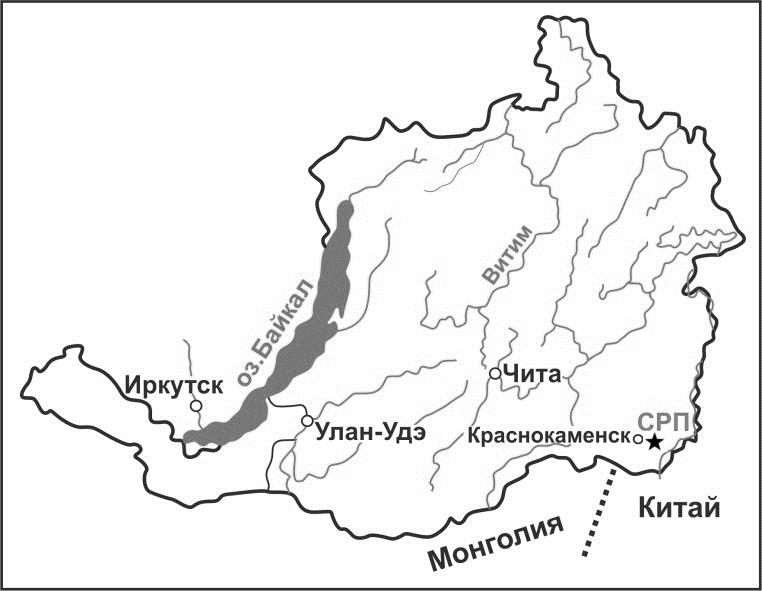
\includegraphics[width=0.5\textwidth]{authors/mandzhieva-fig-1.png}
  \end{center}
  \caption{Схема расположения Стрельцовского рудного поля (СРП)}
  \label{fig:mandzhieva-fig-1}
\end{wrapfigure}


Месторождение Антей, на котором проходила преддипломная практика автора в~составе научной группы ИГЕМ РАН, принадлежит Стрельцовскому рудному полю (СРП), где сосредоточены главные запасы урана России. Оно расположено на юго-востоке Забайкалья в 12~км от г.~Краснокаменск (рис.~1) и включает 19~молибден-урановых месторождений, большая часть которых уникальна по количеству и качеству запасов урана, а также ряд рудопроявлений, ещё не~вовлечённых в эксплуатацию. Работы ведёт Приаргунский горно-обогатительный\,\,\,\,\,\, комбинат\,\,~--- \,\,\,\,основной поставщик урана для нужд атомной промышленности России. Суммарные запасы на момент открытия составляли 250~тыс.~т, это около 73\,\% всего российского урана.

СРП приурочено к Тулукуевской вулкано-тектонической кальдере площадью около 140~км$^2$. В его геологическом строении выделяются два структурных этажа. Нижний сложен протерозойскими и раннепалеозойскими метаморфическими толщами, которые прорваны рифейскими и палеозойскими гранито\-идами. Верхний этаж включает позднеюрские и раннемеловые терригенные и вулканогенные отложения, в которых локализованы средне-позднеюрские малые интрузии и субвулканические тела.

Объектом исследований было урановое месторождение Антей. Оно локализовано в гранитном фундаменте кальдеры. Рудовмещающие породы на месторождении Антей представлены биотитовыми и лейкократовыми гранитами и продуктами их высоко- и низкотемпературных преобразований в рудоносных зонах (рис. 2).

Возраст урановых руд определён на месторождениях Антей и Стрельцовское, прецизионные определения по~ураниниту K-Ar и Rb-Sr методами [13], составил 135\rpm1~млн~лет.

\begin{figure}[H]
  \begin{center}
    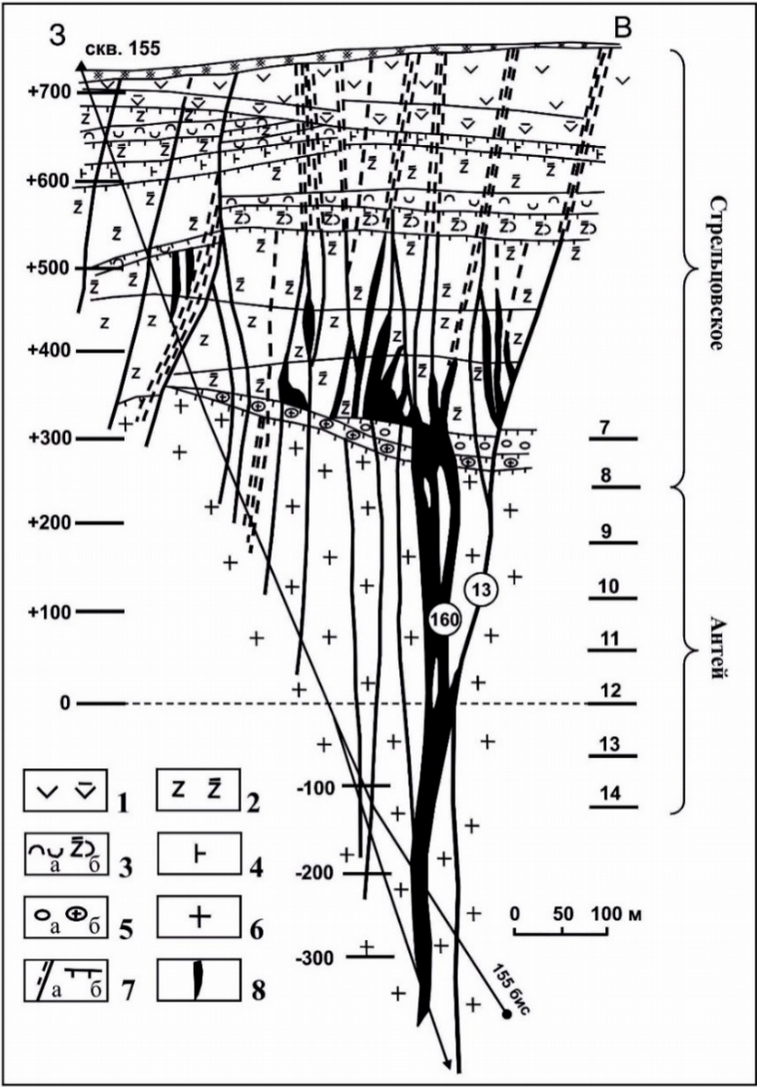
\includegraphics[width=0.75\textwidth]{authors/mandzhieva-fig-2.png}
  \end{center}
  \caption{Разрез по месторождениям Стрельцовское и Антей [5].
Условные обозначения: 1~--- фельзиты; 2~--- трахидациты; 3~--- туфы (а) и туфолавы (б) трахидацитов; 4~--- базальты; 5~--- конгломераты (а) и структурный элювий гранитов (б); 6~--- гранитоиды; 7~--- крутопадающий разлом (а) и пологие срывы (б); 8~--- рудные зоны и отдельные тела. Слева~--- шкала высот над уровнем моря, справа~--- положение в разрезе и номера горизонтов горных выработок}
  \label{fig:mandzhieva-fig2}
\end{figure}


%TODO целью дипломной работы?
Целью исследований было картирование метасоматических преобразований и деформаций рудовмещающих гранитоидов месторождения Антей и~установление зависимости их~петрофизических свойств от глубины и типа метасоматических и деформационных преобразований.

Задачи:
\begin{itemize}[noitemsep]\vspace{-8pt}
  \item отбор ориентированных образцов по горизонтам на месторождении;
  \item построение планов метасоматических преобразований пород по горизонтам месторождения;
  \item проведение структурно-петрофизических исследований (измерение скоростей ультразвуковых волн, гидростатическое взвешивание).
\end{itemize}
 \vspace{-8pt}

В результате наших работ были построены планы горизонтов месторождения, проведена типизация вмещающих гранитоидов, выделены и опробованы объекты для дальнейших детальных структурно-петрофизических и минералого-петрографических исследований. От~этих характеристик напрямую зависят условия проходки подземных выработок и~прогнозирование горных ударов.

Рудовмещающие породы изучали на горизонтах месторождения №~8--13, на глубинах от поверхности 550, 610, 670, 730, 790 и 850~м соответственно. В ИГЕМ РАН автор проводила гидростатическое взвешивание сухих, частично и полностью насыщенных образцов с целью: 1)~определения плотности; 2)~условно мгновенного насыщения; 3)~периода полунасыщения; 4)~эффективной пористости.
Измерялись скорости волн в сухом состоянии после просушивания при температуре 70\,\dgc в течение 4~ч и водонасыщенном, после постепенного погружения в воду до полного насыщения (до момента прекращения увеличения массы) в~течение 7~суток.

Изучение упругих параметров ориентированных образцов в сухом и водонасыщенном состояниях помогает понять строение трещинно-порового пространства породы и предположить механизм миграции рудоносных растворов и местах локализации рудных тел.

В\;\;результате\;\;сравнительного\;\;анализа\;\;выделены\;\;группы\;\;упругих\;\;(модули:\;\;Юнга~Е, сдвига~G, объёмного сжатия~K) и фильтрационно-пористоносных параметров. В результате статистической обработки полученных данных установлено, что петрофизические параметры гранитоидов месторождения Антей значимо различаются в зависимости от характера и интенсивности их разновозрастных высоко- и низкотемпературных гидротермально-метасоматических\;\;\,преобразований,\;\;\,степени\;\;\,тектонической\;\;нарушенности,\;\;особенностей структуры трещинно-порового пространства и совместно с~другими характеристиками могут быть использованы при поисках рудных тел.

Знаток эндогенного уранового оруденения доктор геолого-минералогических наук Георгий Афанасьевич Шатков (ВСЕГЕИ, Санкт-Петербург), выделивший месторождения СРП в самостоятельный генетический тип, пришел к заключению, что основным источником урана здесь выступает специализированный очаг риолитов. При этом наиболее активному выносу урана в гидротермальные растворы способствуют перлитовая и пепловая структуры кислых вулканитов. В ходе ревизии известных рудопроявлений урана на Дальнем Востоке он~обратил внимание на кайнозойские вулканические пеплы Примагаданья и~летом 2014~г. провёл полевые работы на Хасынском и Уптарском месторождениях [14]. Эти образования во многом уникальны, и~представления об их генезисе дискуссионны [3, 6, 7, 9--12, 14]. Детальные лабораторные исследования Г.~А.~Шаткова с соавторами принесли много новых данных, позволивших выдвинуть собственную гипотезу об источнике вулканического материала (очень крупный магматический очаг, находившийся в примагаданской части Центрально-Охотоморского свода). По цирконам, генетически связанным с пеплами, время их формирования отнесено к среднему звену неоплейстоцена (350--140~тыс.~л.~н.). Хотя по~результатам силикатных анализов и структуре РЗЭ магаданские пеплы обнаруживают признаки сходства с перлитами стрельцовского типа, никаких признаков уранового оруденения в них не выявлено. Уникальность магаданских пеплов, по мнению Г.~А.~Шаткова, делает целесообразным сохранение за ними названия <<хасыниты>>, предложенного Е.~Г.~Песковым [7].


\begin{thebibliography}{99}
%1
\bibitem{}\BibAuthor{Алешин~А.~П., Величкин~В.~И., Крылова~Т.~Л.} Генезис и условия формирования месторождения уникального молибден-уранового Стрельцовского рудного поля: новые минералого-геохимические и физико-химические данные // Геология рудных месторождений.~--- 2007.~--- Т.~49, №~5.~--- С.~446--470.
\bibitem{}\BibAuthor{Андреева~О.~В., Головин~В.~А.} Метасоматические процессы на месторождениях Тулукуевской кальдеры в Восточном Забайкалье // Геология рудных месторождений.~--- 1998.~--- Т.~40, №~3.~--- С.~205--220.
\bibitem{}\BibAuthor{Глушкова~О.~Ю., Галанин~А.~А., Смирнов~В.~Н.} Четвертичные вулканические пеплы в Северном Приохотье // Проблемы геологии и металлогении Северо-Востока Азии на рубеже тысячелетий: материалы науч.-практ. конф., посвящ. 100-летию со дня рождения Ю.~А.~Билибина.~--- Магадан~: СВКНИИ ДВО РАН, 2001.~--- Т.~3.~--- С.~14--20.
\bibitem{}\BibAuthor{Дортман~Н.~Б.} Физические свойства горных пород и полезных ископаемых (петрофизика). Справочник геофизика: 2-е изд., перераб. и доп.~--- М.~: Недра, 1984.~--- 455~с.
\bibitem{}\BibAuthor{Ищукова~Л.~П., Авдеев~Б.~В., Губкин~Г.~Н. и др.} Геология Урулюнгуевского рудного района и~молибден-урановых месторождений Стрельцовского рудного поля.~--- М.~: Геоинформмарк, 1998.~--- 382~с.
\bibitem{}\BibAuthor{Мелекесцев~И.~В., Глушкова~О.~Ю., Кирьянов~В.~Ю. и др.} Происхождение и~возраст магаданских вулканических пеплов // Докл. РАН.~--- 1991.~--- Т.~317, №~5.~--- С.~1188--1192.
\bibitem{}\BibAuthor{Песков~Е.~Г.} Геологические проявления холодной дегазации Земли.~--- Магадан~: СВКНИИ ДВО РАН, 2000.~--- 279~с.
\bibitem{}\BibAuthor{Петров~В.~А., Андреева~О.~В., Полуэктов~В.~В.} Влияние петрофизических свойств и деформаций пород на метасоматические процессы в Стрельцовской кальдере (Восточное Забайкалье)~// Докл. РАН.~---  2013.~--- Т.~451, №~2.~--- С.~197.
\bibitem{}\BibAuthor{Сахно~В.~Г., Базанова~Л.~И., Глушкова~О.~Ю. и др.} Происхождение плейстоцен-голоценовых пеплов Северо-Востока России по данным микро- и редкоземельных элементов // Докл. РАН.~--- 2006.~--- Т.~411, №~4.~--- С.~499--504.
\bibitem{}\BibAuthor{Смирнов~В.~Н., Акинин~В.~В., Глушкова~О.~Ю.} Первые определения изотопного возраста вулканических пеплов в кайнозойских отложениях Северного Приохотья // Докл. РАН.~--- 2014.~--- Т.~455, №~6.~--- С.~676--680.
\bibitem{}\BibAuthor{Смирнов~В.~Н., Глушкова~О.~Ю.} Верхнеплейстоценовые ленточные залежи вулканического пепла в Северном Приохотье // Докл. РАН.~--- 2013.~--- Т.~451, №~2.~--- С.~1--5.
\bibitem{}\BibAuthor{Смирнов~В.~Н., Глушкова~О.~Ю., Савва~Н.~Е.} Пеплы камчатских вулканов в районе Магадана\,// Вестник СВНЦ ДВО РАН.~--- 2010.~--- №~1.~--- С.~81--88.
\bibitem{}\BibAuthor{Шатков~Г.~А.} Стрельцовский тип урановых месторождений // Регион. геология и металлогения.~--- 2015.~--- №~63.~--- С.~85--96.
\bibitem{}\BibAuthor{Шатков~Г.~А., Лебедева~О.~Ю., Антонов~А.~В. и др.} Вулканические пеплы Примагаданья: петролого-геохимические особенности и возраст // Регион. геология и металлогения.~--- 2017.~--- №~71.~--- С.~19--34.

\end{thebibliography}
